% \begin{figure}[H]
%     \centering
%     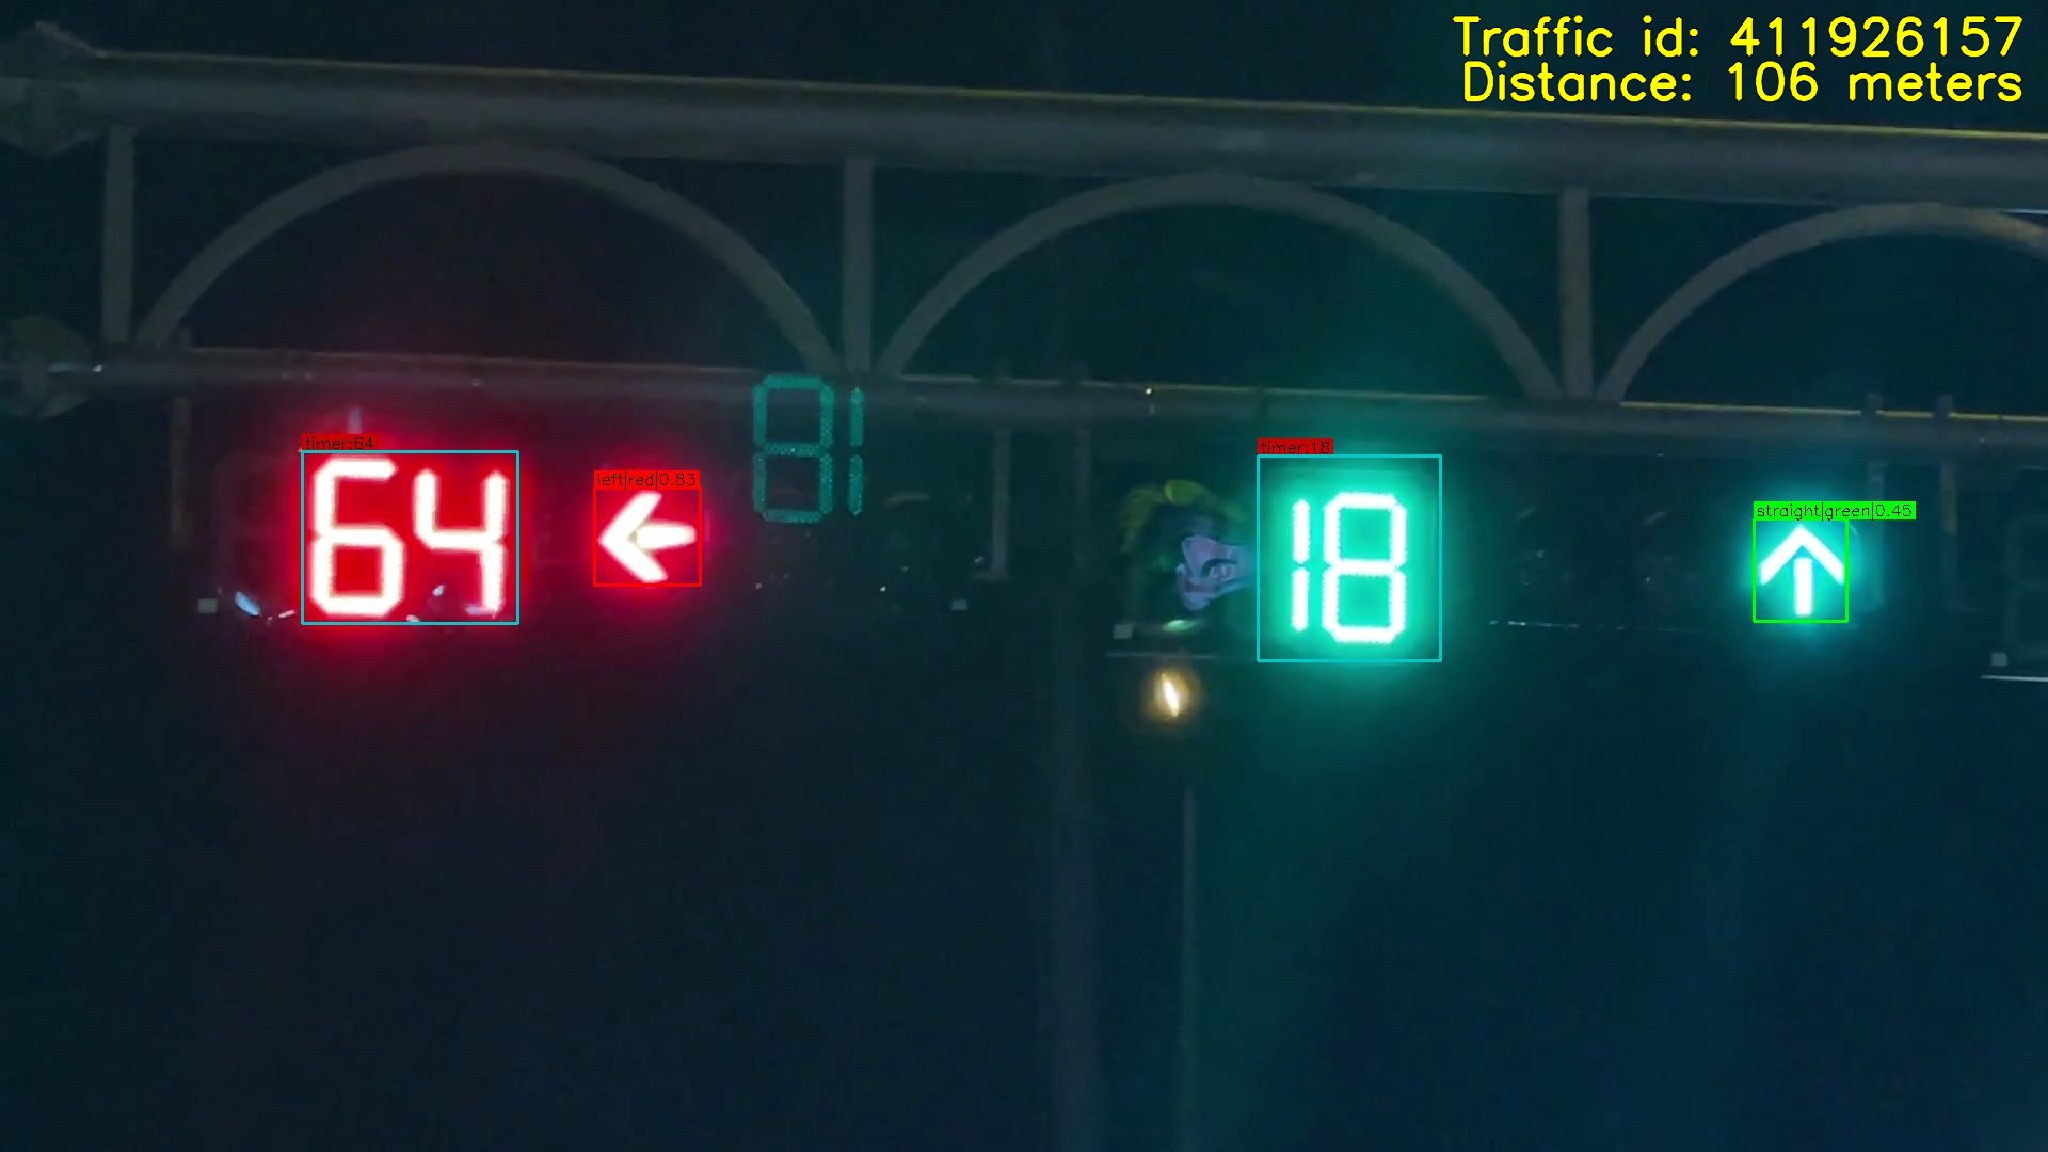
\includegraphics[width=0.75\textwidth]{Images/chapter4/result.png}
%     \vspace{0.5cm}
%     \caption{The result of prototype project}
%     \label{fig:res_project}
% \end{figure}

% Figure~\ref{fig:res_project} illustrates the experimental result obtained from the implemented prototype system. The figure shows the output generated by the ClientSensor application after receiving processed data from the ProviderSensor through the Adaptive AUTOSAR communication mechanism.

% In this experiment, the ClientSensor performs camera-based traffic light detection using the trained YOLO-MobileNet model. Detected traffic lights are highlighted with bounding boxes, and each detection is annotated with the corresponding class label and confidence score, such as red, yellow, and green signal states. The visualization demonstrates that the system is capable of identifying multiple traffic light instances within a single frame and distinguishing different signal colors under indoor test conditions.

% The execution logs displayed in the terminal confirm the end-to-end data flow within the Adaptive AUTOSAR environment. The ProviderSensor successfully publishes processed sensor data, which is then received and consumed by the ClientSensor via SOME/IP with transport protocol (SOME/IP-TP). The logs indicate correct service discovery, data transmission, and event handling between the two applications. Furthermore, the generated output image is stored locally, verifying that the perception results are correctly transferred and processed at the application level.

% Overall, this result validates the functional correctness of the prototype, demonstrating successful integration of deep learning–based perception with Adaptive AUTOSAR service-oriented communication. While the experiment is conducted in a controlled environment and does not represent full automotive deployment conditions, it confirms the feasibility of the proposed architecture and provides a solid foundation for further system optimization and real-world validation.

\subsection{Experimental Setup}
To evaluate the end-to-end functionality of the proposed ADAS architecture followed by the Figure~\ref{fig:archDesign_project}, a hardware-in-the-loop (HIL) experiment was conducted, as previously illustrated in Figure~\ref{fig:hw_arch} in Chapter 2. The setup was designed to simulate a practical in-vehicle network. Specifically, a Raspberry Pi 5 was utilized as the edge computing node to run the Provider application, which handles heavy tasks such as model inference and sensor data collection. A standard USB UVC webcam was connected to capture real-time video streams, while a GPS module supplied accurate vehicle positioning data via a UART interface.
To create a realistic distributed environment, the Client application and the visualization Human-Machine Interface (HMI) were hosted on a separate monitoring computer. This machine was connected to the Raspberry Pi 5 over a Local Area Network (LAN). This separation is important because it ensures that the edge node's processing power is dedicated entirely to AI inference, rather than displaying graphics. 

Furthermore, the overall effectiveness of this setup relies on well-trained perception models. The specific datasets and training configurations used to develop the YOLO26-MobileNetV4 model and the lightweight multi-head CNN timer detector are discussed in detail in Section~\ref{sub:datasetYolo} and Section~\ref{sec:dataCNN}, respectively.

\subsection{System Evaluation}
\begin{figure}[H]
    \centering
    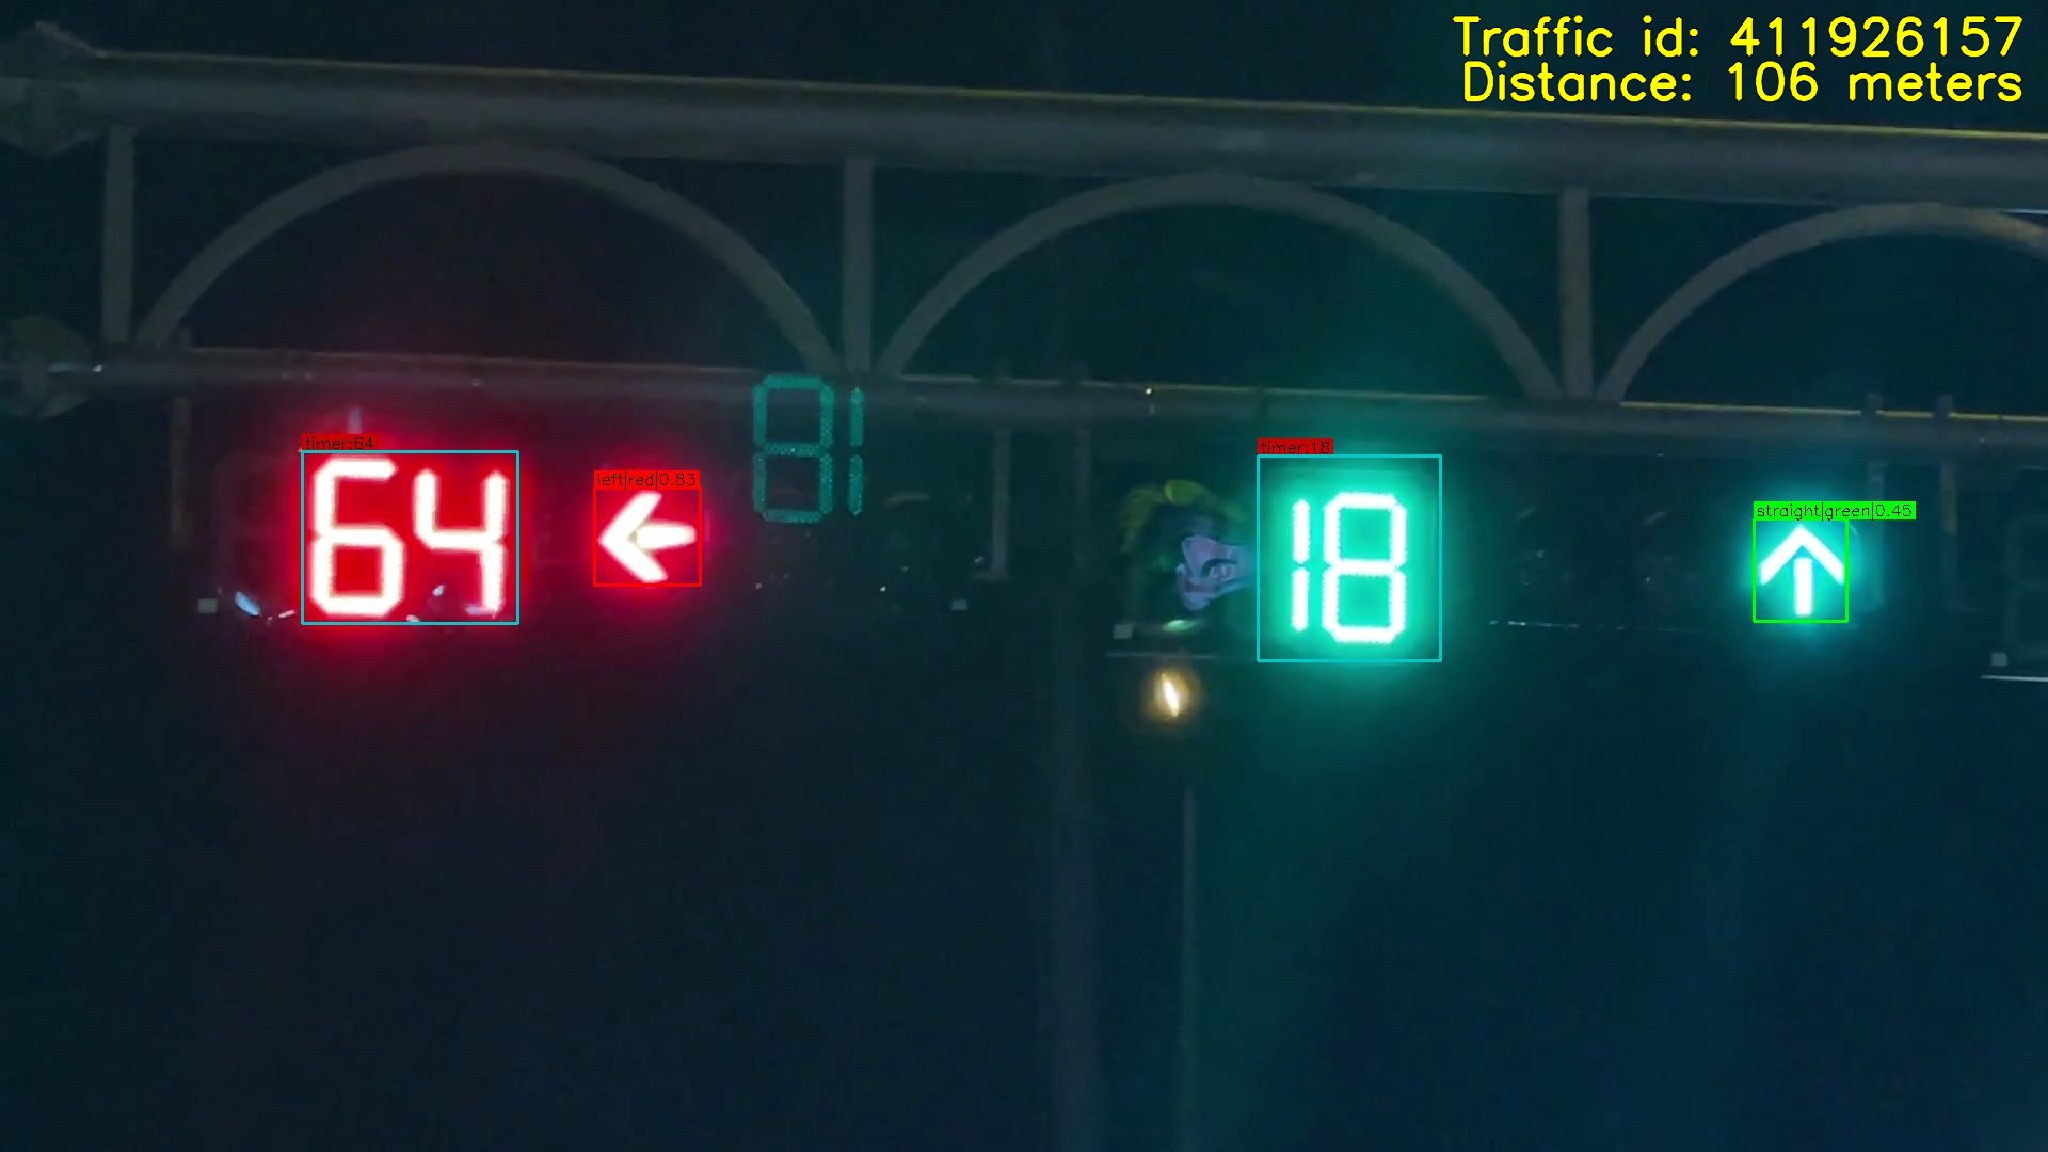
\includegraphics[width=0.75\textwidth]{Images/chapter4/result.png}
    \vspace{0.5cm}
    \caption{Prototype output displayed by the HMI/monitor}
    \label{fig:res_project}
\end{figure}

Figure~\ref{fig:res_project} presents the final visualization produced by the prototype. The monitoring HMI successfully received the data stream from the Client application over the TCP connection. The overlay in the upper-right corner reflects the traffic-light node metadata extracted from the DDS payload, correctly identifying \texttt{Traffic id: 411926157} at a \texttt{Distance: 106 meters}.

During execution, the Provider's perception pipeline successfully captured the camera frame, recognized the traffic light states, and annotated the image. The output highlights a red right-turn signal with a countdown of \texttt{64} seconds and a green straight signal with \texttt{18} seconds remaining. The seamless presentation of both the annotated image and the corresponding GPS metadata confirms that the \texttt{GpsJpegWireHeader} parsing logic functions correctly on the Client side. 

Furthermore, the successful display verifies the reliability of the underlying communication architecture. The \texttt{CycloneDDS-CXX} middleware managed the service discovery and the transportation of the \texttt{imageDataEvent} without observable payload corruption. The experiment demonstrates that the combination of edge-based perception, DDS-driven data distribution, and TCP-based visualization can sustain the required data flow for an ADAS prototype without relying on generic system boilerplates.

With the technical implementations and methodological frameworks thoroughly detailed and validated in Chapter 4, the primary objectives of this research have been addressed. Transitioning into Chapter 5, the focus will shift towards a final synthesis of the project. The upcoming chapter will offer a conclusive summary of the findings, reflect on the practical implications of the developed ADAS system, and propose viable recommendations for future enhancements.